\documentclass{article}
\usepackage{graphicx}
\usepackage{amsmath}
\usepackage{hyperref}

\title{Project 2: Hybrid Sorting Algorithms}
\author{Rachel Koch}
\date{\today}

\begin{document}
	
\maketitle

\section{Attributions}

ChatGPT file changes: \textit{project2.py}
\begin{quote}
\textbf{Overall Code Changes} \\
Import sys library \\
Reorganized code so it is in order of deliverable \\
Changed the names of the sorting algorithms to match the docs \\
Added console messages indicating successful activities \\
Added comments to functions \\
Added a value of n and increased the other experiment values \\
Increased the upper limit and step size on K \\
VerificationTest results get sent to a file

\textbf{New Functions} \\
Added a verificationTest function to test my sorting algorithm \\
Added a newIntArray function to generate arrays of random ints

\textbf{InsertionSort function} \\
Stored length of array in variable $n$ \\
Added a check for array of length zero/one 

\textbf{Merge function} \\
Added an if-statement to check which array was emptied first

\textbf{run\_time\_experiment function} \\
Used newIntArray function to generate integer arrays

\textbf{plot\_results function} \\
Moved the legend next to the plot instead of on it \\
Figure box size changed to fit legend
\end{quote}

ChatGPT file changes: \textit{project2\_report.tex}

\begin{quote}
Section for Deliverable 1 now shows algorithm and tests/approach \\
Different graph in Deliverable 2 because different values were used \\
Discussion in Deliverable 2 was adjusted to match the new figure \\
Changed the graph and observations in Deliverable 3 \\
Graphs and discussion in Deliverable 4 were changed \\
Added a conclusion
\end{quote}
	
\section*{Deliverable 1: Implementation and Verification of Correctness}

\subsection{Algorithm}
This project implemented the HybridSort algorithm by combining MergeSort and InsertionSort. The algorithm includes:
	
\begin{itemize}
    \item \textbf{InsertionSort}: For sorting small arrays.
    \item \textbf{Merge}: For merging two sorted arrays.
    \item \textbf{HybridSort}: Switches between MergeSort and InsertionSort based on a threshold \( K \).
\end{itemize}
	
\subsection{Verification}
Verification test results can be found in a file named \textit{test.txt}. Each test generated an array of random integers and compared the sorting results of both HybridSort and the python sorting algorithm, indicating a pass/fail. We fixed K at 5 for verification testing, and limited the arrays to 50 integers or less. Testing showed that the HybridSort algorithm results and the Python sorted(list) function results matched in every case. By the end of this project, over 90 tests had been performed and they all passed. A small subset of the results are shown below. \\ \\
\ttfamily
Verification Test \\
$[$7, 98, 79, 17, 76, 1, 2, 55, 58, 22, 99, 97, 54, 93, 82, 50, 56, 43$]$ \\
Passed \\
K = 5 \\
Hybrid =  $[$1, 2, 7, 17, 22, 43, 50, 54, 55, 56, 58, 76, 79, 82, 93, 97, 98, 99$]$ \\
Sort =  $[$1, 2, 7, 17, 22, 43, 50, 54, 55, 56, 58, 76, 79, 82, 93, 97, 98, 99$]$ \\
\\
Verification Test \\
$[$53, 95, 57, 53, 69, 24, 28, 53, 71, 76, 0, 73, 49, 39, 12, 27, 74, 52, 23, 53, 5, 12, 50, 58, 57, 29, 70, 9, 41, 64, 7$]$ \\
Passed \\
K = 5 \\
Hybrid =  $[$0, 5, 7, 9, 12, 12, 23, 24, 27, 28, 29, 39, 41, 49, 50, 52, 53, 53, 53, 53, 57, 57, 58, 64, 69, 70, 71, 73, 74, 76, 95$]$ \\
Sort =  $[$0, 5, 7, 9, 12, 12, 23, 24, 27, 28, 29, 39, 41, 49, 50, 52, 53, 53, 53, 53, 57, 57, 58, 64, 69, 70, 71, 73, 74, 76, 95$]$ \\
\\
Verification Test \\
$[$29, 78, 28, 32, 85, 18, 25, 81, 6, 45, 79, 44$]$ \\
Passed \\
K = 5 \\
Hybrid =  $[$6, 18, 25, 28, 29, 32, 44, 45, 78, 79, 81, 85$]$ \\
Sort =  $[$6, 18, 25, 28, 29, 32, 44, 45, 78, 79, 81, 85$]$ \\
\\
Verification Test \\
$[$7, 24, 60, 96, 0, 91, 97, 3, 22, 50, 12, 17, 87, 87, 92, 5, 38, 10, 10, 43$]$ \\
Passed \\
K = 5 \\
Hybrid =  $[$0, 3, 5, 7, 10, 10, 12, 17, 22, 24, 38, 43, 50, 60, 87, 87, 91, 92, 96, 97$]$ \\
Sort =  $[$0, 3, 5, 7, 10, 10, 12, 17, 22, 24, 38, 43, 50, 60, 87, 87, 91, 92, 96, 97$]$ \\
\\
Verification Test \\
$[$58, 1, 37, 33, 11, 38, 61, 45, 34, 24, 29, 20, 4, 32, 26, 78, 93, 8, 83, 7, 57, 27, 47, 12, 76, 16, 64, 2, 68, 5, 84, 90, 66, 90, 59, 36, 81, 68, 33, 27, 18, 33, 97, 33, 12, 97$]$ \\
Passed \\
K = 5 \\
Hybrid =  $[$1, 2, 4, 5, 7, 8, 11, 12, 12, 16, 18, 20, 24, 26, 27, 27, 29, 32, 33, 33, 33, 33, 34, 36, 37, 38, 45, 47, 57, 58, 59, 61, 64, 66, 68, 68, 76, 78, 81, 83, 84, 90, 90, 93, 97, 97$]$ \\
Sort =  $[$1, 2, 4, 5, 7, 8, 11, 12, 12, 16, 18, 20, 24, 26, 27, 27, 29, 32, 33, 33, 33, 33, 34, 36, 37, 38, 45, 47, 57, 58, 59, 61, 64, 66, 68, 68, 76, 78, 81, 83, 84, 90, 90, 93, 97, 97$]$ \\
\\
\rmfamily
Additional test results are appended to the original \textit{test.txt} file every time the program is run, so testing can be independently verified. Screenshots are included to show that the file contained 95 passed tests and no failed tests. 
    \begin{figure}[h!]
	\centering
	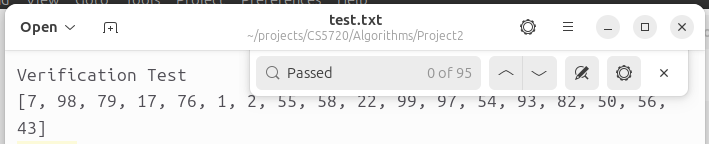
\includegraphics[width=\textwidth]{Screenshot from 2024-10-25 23-15-03.png}
	\caption{Screenshot showing 95 passed tests.}
    \end{figure}
    
    \begin{figure}[h!]
	\centering
	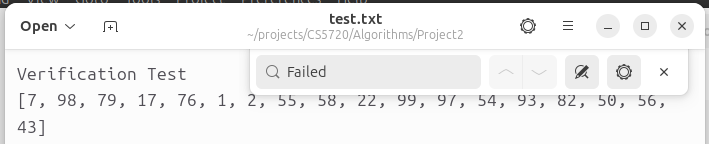
\includegraphics[width=\textwidth]{Screenshot from 2024-10-25 23-15-16.png}
	\caption{Screenshot showing 0 failed tests.}
    \end{figure}
	
\section*{Deliverable 2: Average Running Time vs. K (Random Arrays)}
\textbf{Note:} Definitive performance metrics on this algorithm will depend on the computer used for testing. This is due to variables such as cache size, processor speed, memory capacity, predictive modeling, etc. \\

Experiments were conducted on randomly generated arrays of various sizes \( n \) and the average running time of HybridSort was measured for different values of \( K \). The results are shown in Figure \ref{fig:random}.
	
\begin{figure}[h!]
    \centering
    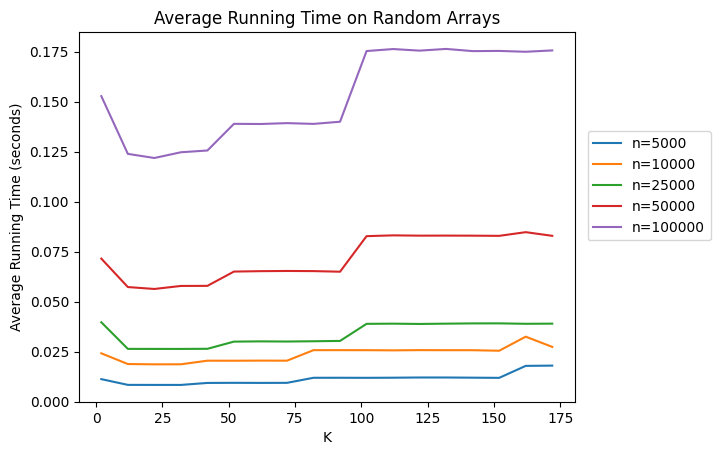
\includegraphics[width=\textwidth]{random_results.png}
    \caption{Average Running Time of HybridSort on Random Arrays.}
    \label{fig:random}
\end{figure}

As seen in this figure, the running time decreases initially as \( K \) increases, but at larger values of \( K \), the running time increases again (to worse than it started). This indicates, as expected, that small values of \( K \) are inefficient because they invoke MergeSort too often, whereas large values of \( K \) are inefficient because they overuse InsertionSort. This effect becomes more pronounced for larger values of $n$.

\section*{Deliverable 3: Optimal K as a Function of Array Length (Random Arrays)}
	
An optimal \( K \) value was identified for each array size \( n \) by selecting the \( K \) value that resulted in the fastest running time. The relationship between \( n \) and optimal \( K \) is shown in Figure \ref{fig:optimal_k}.
	
\begin{figure}[h!]
    \centering
    \includegraphics[width=\textwidth]{optimal_k.png}
    \caption{Optimal K for Different Array Sizes (Random Arrays).}
    \label{fig:optimal_k}
\end{figure}

The results shown in Figure \ref{fig:optimal_k} can be affected by adjusting the step size of K and the content of the input arrays - which were defined in the experiments for Deliverable 2. Particularly for smaller values of $n$, the random integers that are generated to fill the arrays have a high impact on this part of the analysis. Meaning that the distribution of integers seems to determine how effective InsertionSort is. If the distribution is favorable, then InsertionSort can operate faster on larger arrays. This has a higher impact on small $n$ because variations aren't easily drowned out by the multitudes of other measurements. However, for large values of $n$, the optimal $K$ value was easier to determine, and typically settled at 22. 

I ran through this exercise multiple times - changing and not changing settings - but my results varied more than expected. Sometimes all the optimal $K$ values landed at $K= 22$, making the evaluation easy. In other iterations, the $K$ values for smaller $n$ were anything from $K= 10$ to $K = 32$, due to a variety of integer distributions. I even had instances where the optimal $K$ values for larger $n$ were not consistent. Generally, though, the optimal values for $K$, at larger values of $n$, were stable, because variations due to integer distribution were averaged out across many measurements. This indicates that while the leader appears to be $K=22$, a precise optimal $K$ value (especially for small $n$) depends on the distribution of integers in a given situation. 

\section*{Deliverable 4: Average Running Time vs. K (Sorted Arrays)}
	
The experiments from Deliverables 2 and 3 were repeated with pre-sorted arrays. Results of these average running time experiments are shown in Figure \ref{fig:sorted}.
	
\begin{figure}[h]
    \centering
    \includegraphics[width=\textwidth]{sorted_results.png}
    \caption{Average Running Time of HybridSort on Sorted Arrays.}
    \label{fig:sorted}
\end{figure}
	
\textbf{Differences with Random Arrays}: As expected, the overall running times of HybridSort are much faster on sorted arrays. This is because InsertionSort runs in $\Theta(n)$ time on sorted arrays, making the algorithm run faster than before for every value of $K$. Unlike in Figure \ref{fig:random}, there is no clear threshold on Figure \ref{fig:sorted} where the algorithm starts to run worse for larger $K$, even for larger $n$, because that threshold is where InsertionSort starts to run less efficiently, which doesn't happen here. When the array is pre-sorted, InsertionSort always runs at its most efficient, regardless of the array size. The initial running times in Figure \ref{fig:sorted} are slower for small $K$, as was also seen on the random arrays in Figure \ref{fig:random}, but this is due to the fact that MergeSort has to run more often in these cases, making the overall run time slower. 
	
\section*{Deliverable 4 (Continued): Optimal K as a Function of Array Length (Sorted Arrays)}
	
The optimal \( K \) value analysis was also repeated using only sorted arrays. These optimal values of \( K \) are shown in Figure \ref{fig:optimal_k_sorted}.
	
\begin{figure}[h]
    \centering
    \includegraphics[width=\textwidth]{optimal_k_sorted.png}
    \caption{Optimal K for Different Array Sizes (Sorted Arrays).}
    \label{fig:optimal_k_sorted}
\end{figure}
	
\textbf{Differences with Random Arrays}: In contrast to random arrays, the optimal \( K \) values for sorted arrays are much larger, as can be seen in Figure \ref{fig:optimal_k_sorted}. After running these tests multiple times, most of the optimal $K$ values landed at whatever the largest tested $K$ value was - because InsertionSort was always running most efficiently, regardless of array size. Occasionally, some earlier values of $K$ would qualify as optimal, which can be seen in Figure \ref{fig:optimal_k_sorted}, but the difference in runtimes was minimal ($\leq 0.0001$ seconds faster). This is very different than what was found in Figure \ref{fig:optimal_k}, where the efficiency of InsertionSort depended heavily on the distribution of the random integers, but tended to stabilize around a low value of $K$. In Deliverable 3, it was less efficient to use InsertionSort for larger arrays, but in the case of sorted arrays, the array size didn't affect the efficiency of InsertionSort, making it efficient to use InsertionSort as often as possible.  \\

\section*{Conclusion}
This project found that HybridSort was most efficient on sorted arrays, but still pretty fast on random arrays if the correct $K$ value was chosen. In the case of our sorted arrays, InsertionSort is known to run in $\Theta(n)$ time, making it fast and most efficient every time it ran. MergeSort runs in $\Theta(n \log n)$ time, which is slower than $\Theta(n)$ time. This explains why, when the array was pre-sorted, it was always most efficient to use InsertionSort for as large an array as was allowed. On random arrays though, InsertionSort runs in $\Theta(n^2)$ time on average, making it less efficient to use InsertionSort as often, and more efficient to call MergeSort earlier. The combination, though, of InsertionSort and MergeSort, still performed better than either one by itself, in every case. 
	
\end{document}
